\chapter{Regression \label{chapter:regression}}

Classification is a form of supervised learning in which the outcome is a category. \textbf{Regression}\index{regression} is another form of supervised learning in which the outcome is a numeric value. For example, it may be a lab value, physical characteristic (height, weight, etc.), or numeric measurement (e.g. oxygen saturation).

%%%%%%%%%%%%%%%%%%%%%%%%%%%%%%%%%%%%%%%%%%%%%%%%%%%%%%%%%%%%%%%%%%%%%%%%%%%%%%%%%%%%%%

\section{Visualizing the Regression Problem \label{section:visualizingreg}}

Let's consider the same setup from Section~\ref{section:visualizingclass} but this time with a quantitative outcome: a ``recurrence biomarker'' that indicates the likelihood of recurrence of disease.

Again, we have data on two predictors: a disease severity score ($x_1$), which characterizes the severity of the illness for which the patient was originally treated, and a social determinants score ($x_2$), which characterizes a patient's socioeconomic status. We have measurements of $x_1$ and $x_2$ on the same $200$ patients as in Section~\ref{section:visualizingclass}. 

\begin{center}
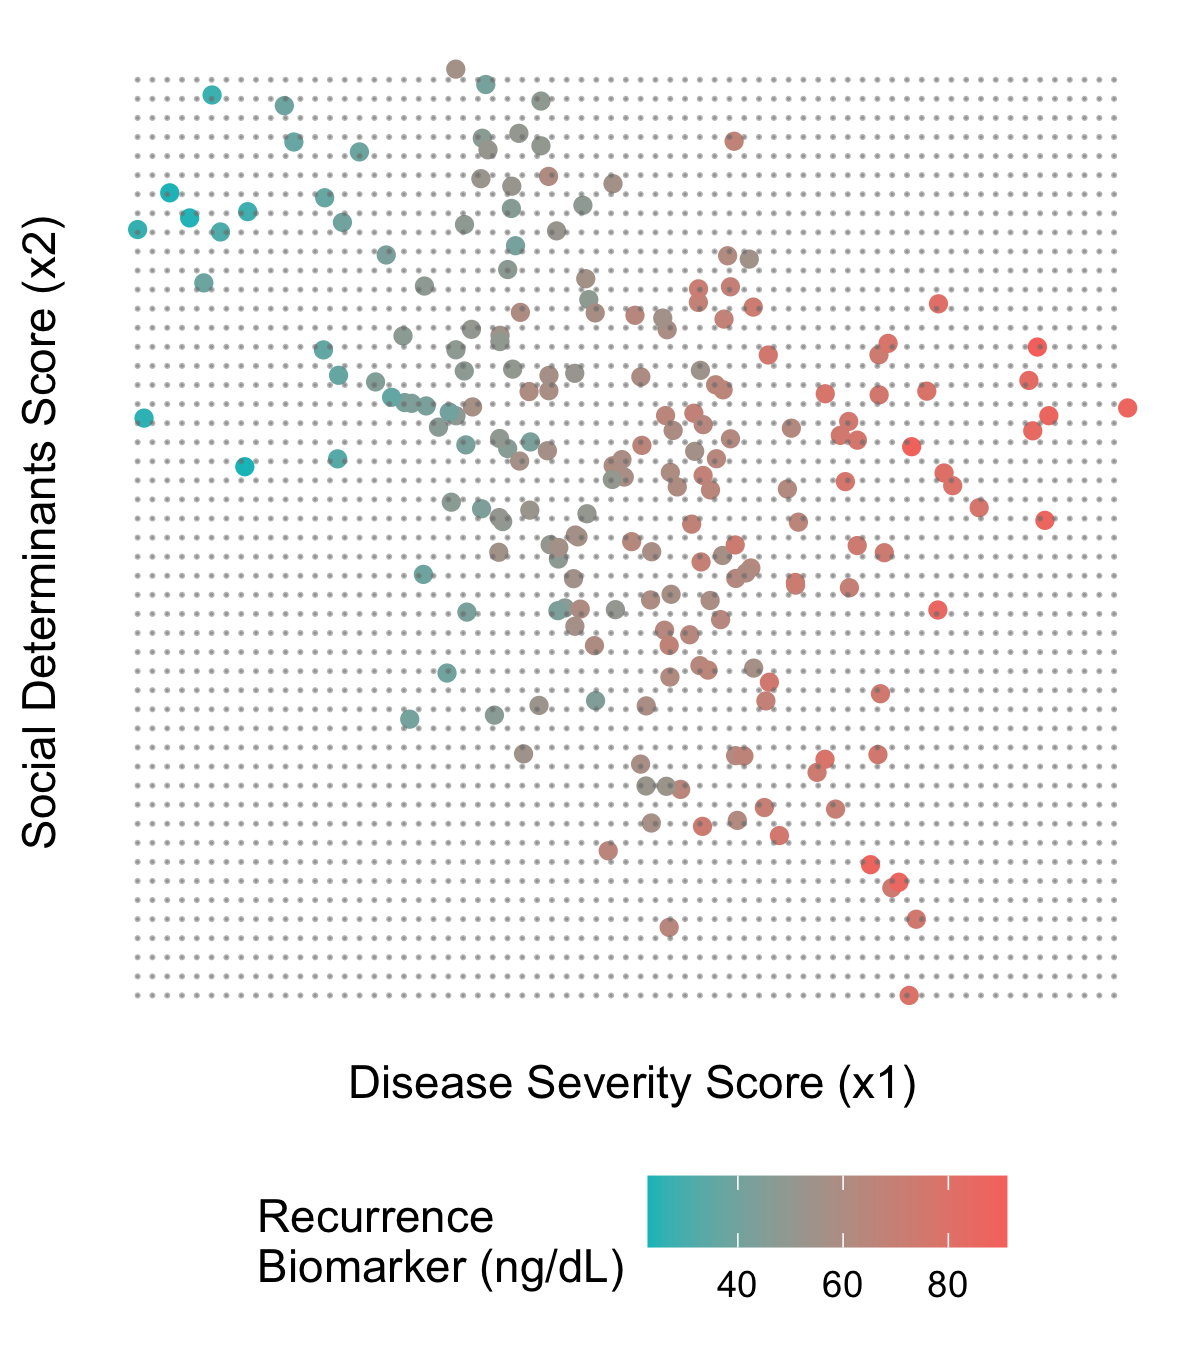
\includegraphics[width=0.7\textwidth]{img/esl-reg-just-data.png}
\end{center}

This is a plot of the data in a single plane. The color represents the value of the recurrence biomarker -- the height of the point above the plane. The goal of regression is to predict the value of the biomarker ($y$) based on the values of the two predictors, $x_1$ and $x_2$.
\vspace{5mm} 

\begin{question}{question:influence}
Just looking at the two predictors, which one appears to more highly influence the value of the recurrence biomarker? Why?
\end{question}

\begin{question}{}
Think about the three algorithms we discussed in Chapter~\ref{chapter:classification}. Now think about our new task, which is to predict the \emph{numeric value} of the recurrence biomarker as a function of the two predictors, $x_1$ and $x_2$. 
\begin{itemize}
\item How might you adapt KNN to deal with this problem?
\item How might you adapt a decision tree to deal with this problem?
\item How might you adapt logistic regression to deal with this problem? You'll have to ``break the algorithm'' a bit more this time.  
\end{itemize}
\end{question}

%%%%%%%%%%%%%%%%%%%%%%%%%%%%%%%%%%%%%%%%%%%%%%%%%%%%%%%%%%%%%%%%%%%%%%%%%%%%%%%%%%%%%%

\section{Three Regression Algorithms}

\subsection{Linear Regression \label{ssect:linreg}}

The regression analogue of logistic regression is \textbf{linear regression}\footnote{The terminology here is confusing. When we learn about generalized linear models in Chapter~\ref{chapter:glms}, you'll see why logistic regression has the word ``regression'' in its name even though it's a classification algorithm.}. Linear regression creates a hyperplane that slices through the cloud of training datapoints such that it passes as close as possible, on average, to the data. This is, of course, easiest to see when the feature space is two-dimensional, as it is here:

\begin{center}
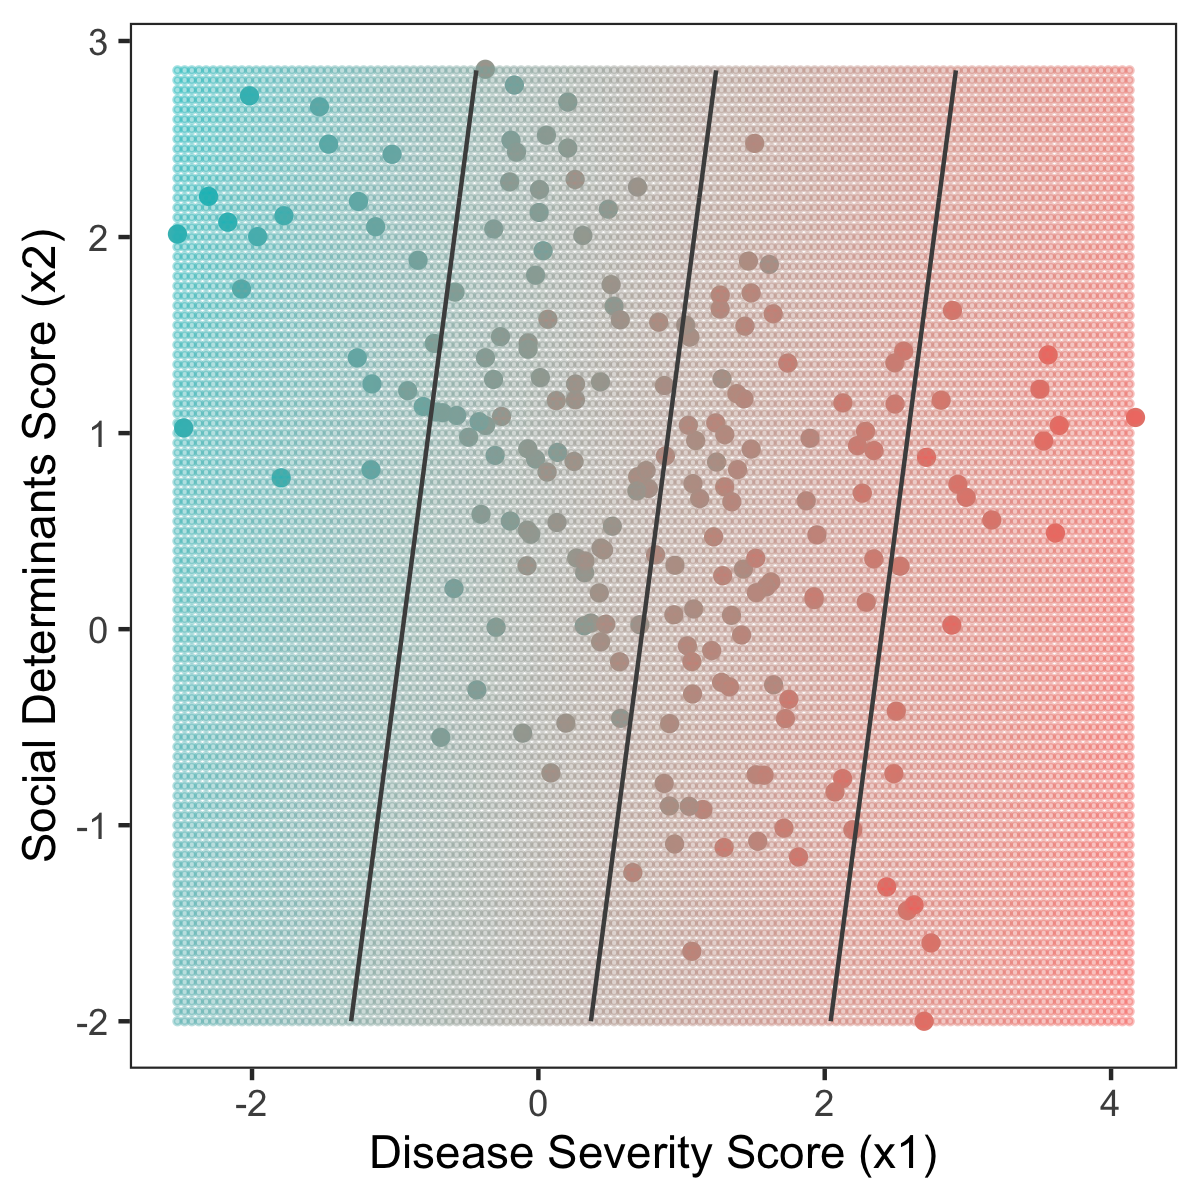
\includegraphics[width=0.7\textwidth]{img/esl-reg-linear.png}
\end{center}
The three lines shown here sit on the hyperplane learned by the linear regression model. They are located at heights corresponding to the 25th, 50th, and 75th percentiles of the outcome, $y$ (the biomarker value). The plane tilts downward toward the upper left corner of the $x_1 \times x_2$ grid and upward toward the bottom right corner. It may be helpful to visualize grabbing the $x_1 \times x_2$ plane and rotating/translating it so that it passes through the middle of the training data.   

\subsection{K Nearest Neighbors (KNN)}

Regression using KNN works very similarly to KNN for classification. In classification, we allow the nearest $K$ points to vote on the label of a new test point. In regression, we \textbf{interpolate} between the values of the surrounding points to come up with the value of $y$ for a test point. Typically this is done just by averaging the $y$ values of the nearest $K$ points, but you can also do something more sophisticated, like weight their contributions by distance to the test point. Here is a contour plot of the regression surface produced by KNN ($K=15$) for our example:

\begin{center}
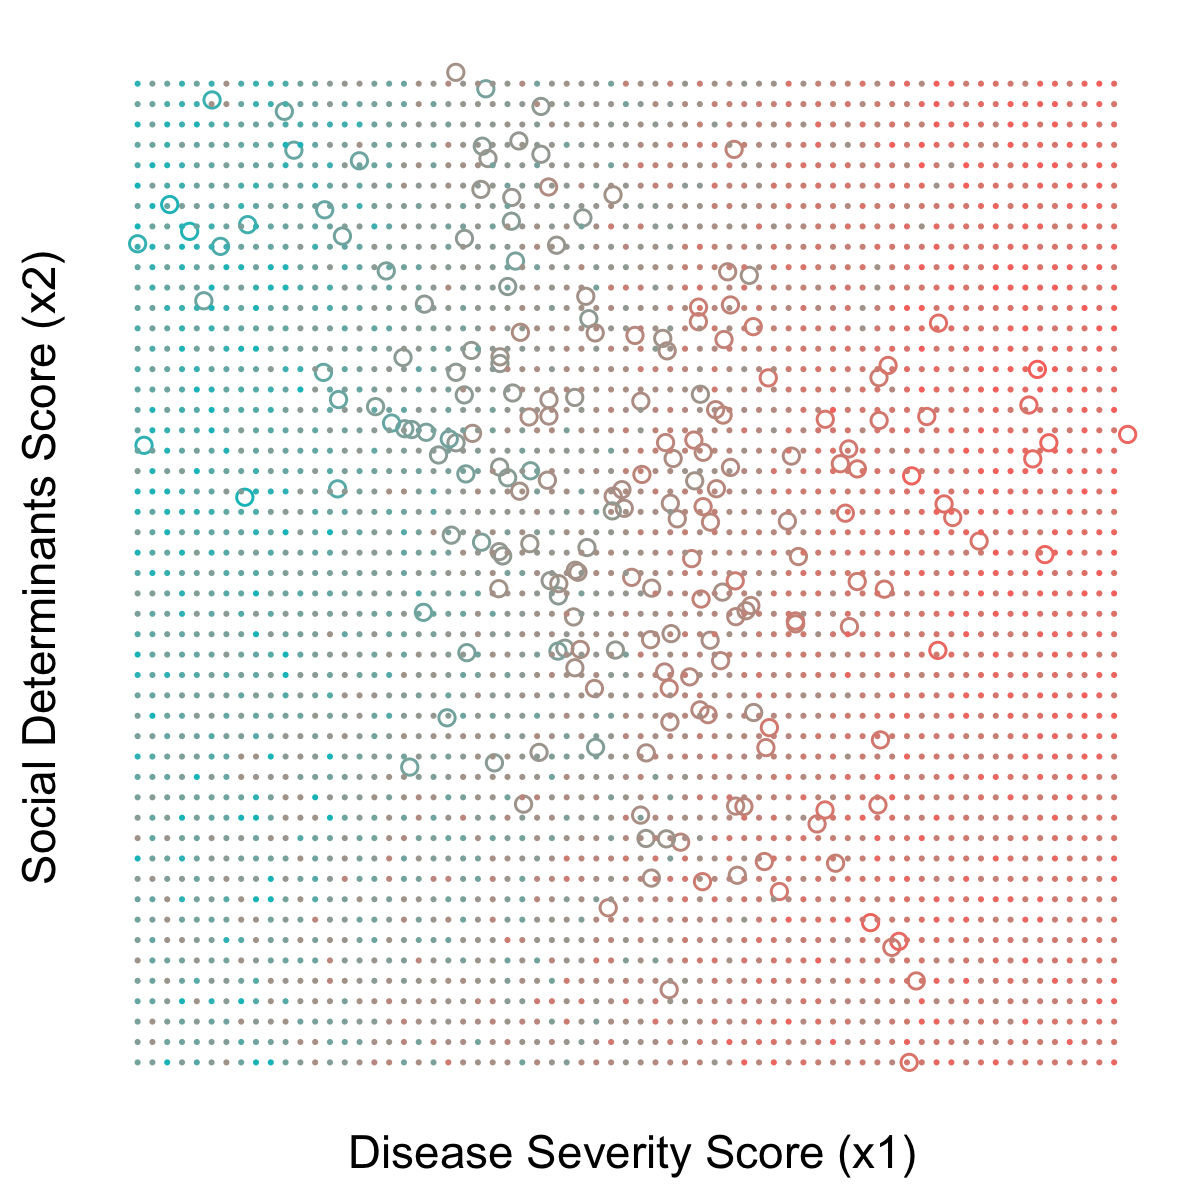
\includegraphics[width=0.7\textwidth]{img/esl-reg-knn-15.png}
\end{center}

\noindent The contours are again drawn at the 25th, 50th, and 75th percentiles of the outcome, $y$. This looks like a bit of a mess compared to the linear regression plot, but at the same time, the KNN algorithm is able to capture arbitrarily complex relationships between $x_1$, $x_2$, and $y$ that can be missed by other regression algorithms.  

\subsection{Decision Tree}

Decision tree regression is similar to decision tree classification except that the output at each leaf is not a class label or the probability of membership in the positive training class (both of which are shown on the tree in Section~\ref{ssect:class_decision_tree}), but a numeric value. That value corresponds to the mean outcome value for the points in that leaf. 
\begin{center}
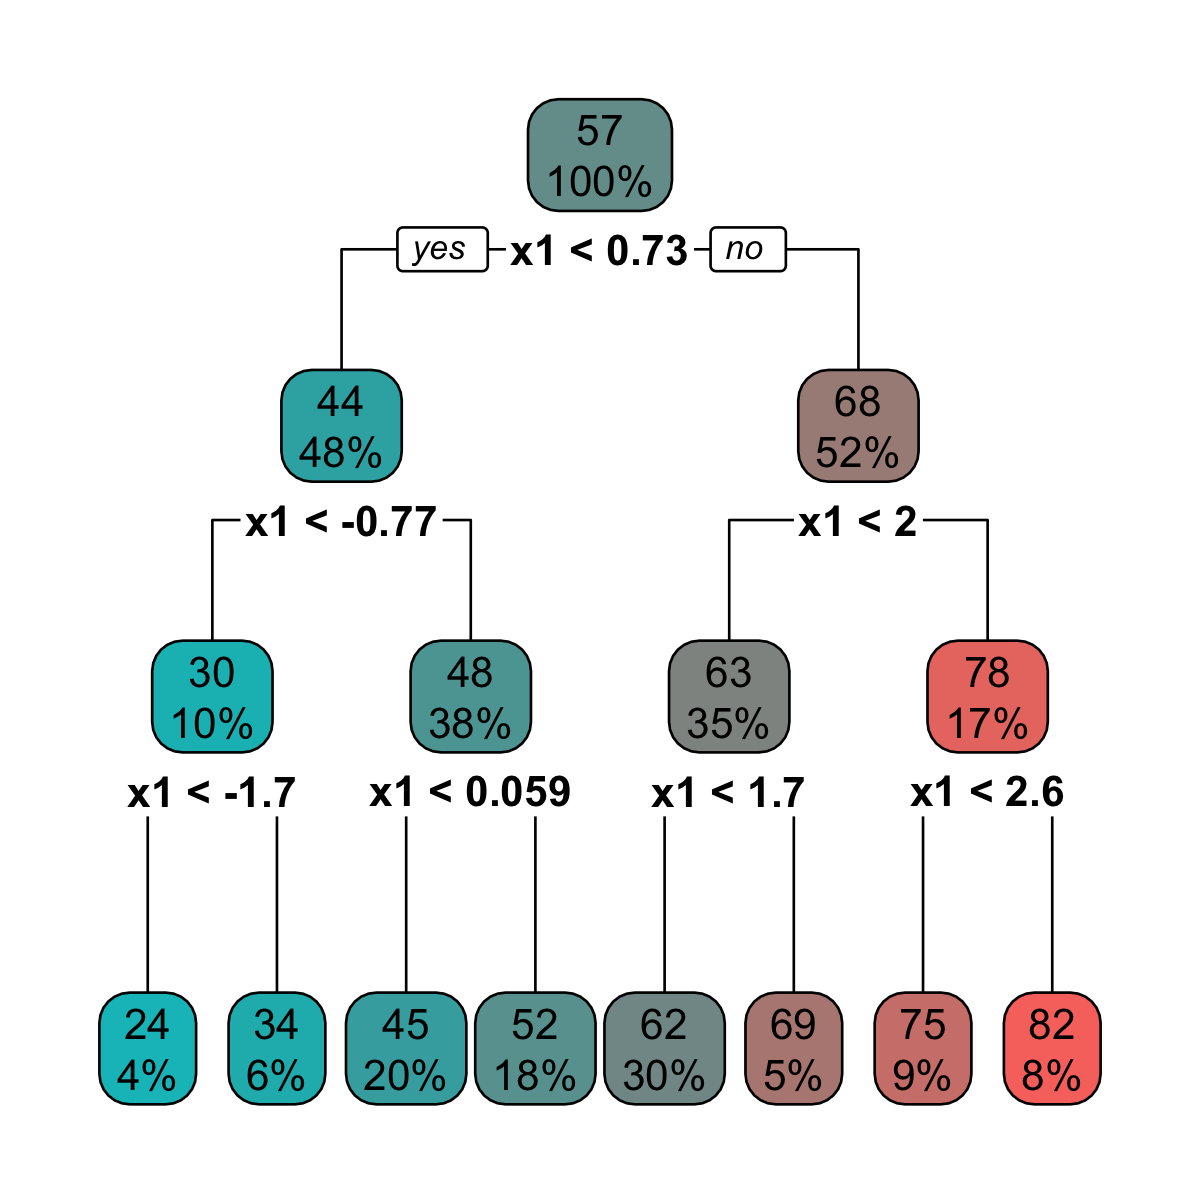
\includegraphics[width=0.6\textwidth]{img/esl-decision-tree-just-tree-reg.png}
\end{center}
The predicted biomarker values for a decision tree trained on this dataset (created using the \texttt{rpart} package in R with default parameters) are shown here:
\begin{center}
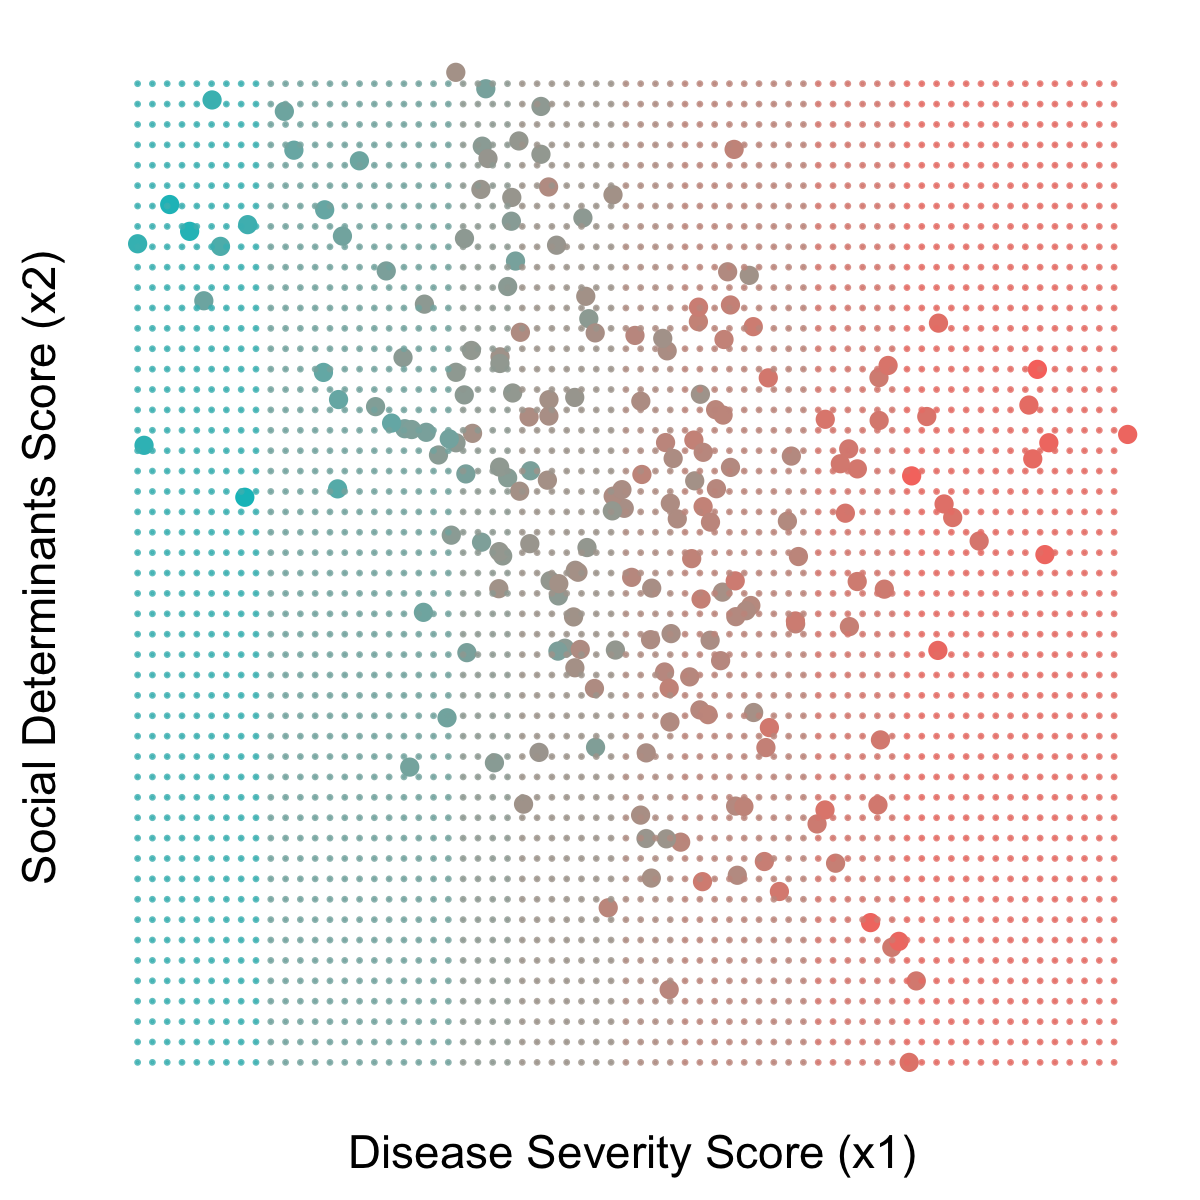
\includegraphics[width=0.7\textwidth]{img/esl-reg-decision-tree.png}
\end{center}
You can see that the decision tree always chooses to split on $x_1$, the disease severity score, rather than $x_2$. Revisit Question~\ref{question:influence} to remind yourself of why this is. The regression surface produced by the decision tree looks like a set of stairs climbing higher and higher as one moves from left to right across the $x_1 \times x_2$ plane. Of course, it would be difficult to climb such stairs, because they are not evenly spaced!
\vspace{5mm}

\begin{question}{}
What are the advantages and disadvantages of each of these three regression algorithms?
\end{question}

